\chapter{深層状態空間モデルの限界}
\label{chap:baseline}


深層状態空間モデルは,潜在変数の次元を大きくしたときの学習が難しい.そのことを実験的に示した上で、理論的な問題点を述べる.

\section{学習が失敗した例}
\ref{fig:dssm_failure}は、本論文の4章以降でベースラインとして述べる通常のSSMモデルを、潜在変数の次元を何通りかに変えてモデルを構築し、学習中の様子ある.潜在変数を低次元にすると順調に学習が進み、少しずつ近い映像が出力されるようになるが,次元を大きくすると途中で目的関数とする変分下限の値が正の方向に発散しやすくなる.さらに調べると、変分下限の2つの項のうち、KLダイバージェンスが先に発散していることがわかる.

% \caption[hoge]{fuga}
\begin{figure}[tbp]
    \begin{center}
      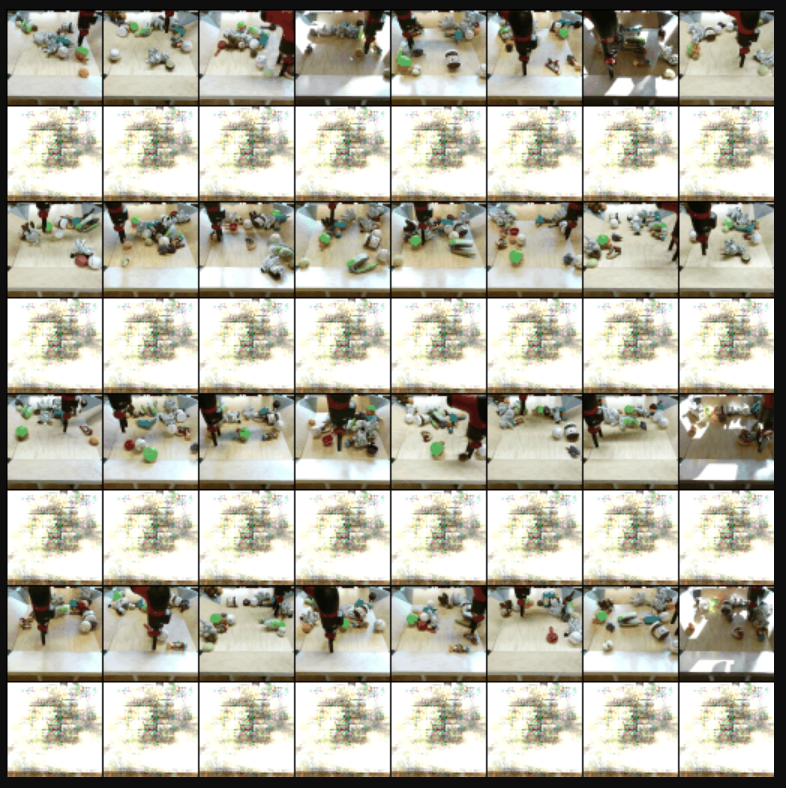
\includegraphics[width=\linewidth]{./figures/dssm_failure.png}
      \caption{DSSMの学習が失敗した例}
      \label{fig:dssm_failure}
    \end{center}
  \end{figure}

\section{深層状態空間モデルの問題点}
\begin{eqnarray}
  \end{eqnarray}
  
\begin{eqnarray}
    (VAEのELBO) \nonumber = \mathbb{E}_{\bm{z} \sim q(\bm{z}|\bm{x})} [\log p(\bm{x}|\bm{z})] - \mathrm{D_{KL}}(q(\bm{z}|\bm{x}) \| p(\bm{z})) \label{eq:vae_elbo2} \\
\end{eqnarray}
\begin{eqnarray}
    \ (DSSMのELBO) \nonumber \\
    &=& \sum_{t=1}^T \left( \mathbb{E}_{s_t \sim q(s_t|a_{1:t}, o_{1:t})} [\log p(o_t|s_t)] \right. \nonumber \\
    && \hspace{2em} \left. - \mathbb{E}_{s_{t-1} \sim q(s_{t-1}|a_{1:t-1}, o_{1:t-1})} [\mathrm{D_{KL}}(q(s_t|s_{t-1}, a_t, o_t) \| p(s_t|s_{t-1}, a_t, o_t))] \right)  \nonumber \\
    \label{eq:dssm_elbo2}
  \end{eqnarray}

VAEではこのような問題は起きない。
DSSMで学習が難しい理由として、以下が考えられる
1VAEと違い、DSSMではKL項でpriorを近づけ先であるposteriorが固定されていない.
2stateの次元が小さく、$H(o) >> H(s_{prev})$ であるときのposteriorの出力は一意に定まり
stateの次元が大きく $H(o) >> H(s_{prev})$でない時は安定しない
近似がゆるくなる!!!!!
また、stateの推論にモンテカルロ近似をするが、その時のサンプル回数Lを増やすて平均を取ることは、経験的にうまく行かないことが知られてたりするのかな…?

近づけ先が固定されていないときにKLがnanすることは、Variational Autoencoder with Arbitrary Conditioningなどでも言われている
